\documentclass[11pt]{article}
\usepackage{graphicx}
\usepackage{booktabs}
\usepackage{amsmath}
\usepackage{hyperref}
\usepackage{geometry}
\usepackage{float}
\geometry{margin=1in}

\title{Online vs.\ Offline Learning: \\
       A Comparative Empirical Analysis of \\
       Exam Performance, Retention, and Focus}
\author{Researcher}
\date{\today}

\begin{document}
\maketitle

\begin{abstract}
The rapid expansion of online education has prompted renewed interest in understanding how the
learning modality---online versus offline---affects academic outcomes.
This study presents a comparative empirical analysis of 1,000 students
(500 online, 500 offline) drawn from five subject areas: Science, English, History, Math,
and Programming.
Four outcome variables are examined: Exam Score, Retention Score, Focus Level, and
Study Hours.
Independent-samples $t$-tests and Mann-Whitney $U$ tests reveal that offline learners
score significantly higher on both Exam Score ($\bar{x}_{\text{off}} = 73.14$
vs.\ $\bar{x}_{\text{on}} = 70.21$; $t = -3.579$, $p = 0.0004$) and
Retention Score ($\bar{x}_{\text{off}} = 74.72$ vs.\ $\bar{x}_{\text{on}} = 70.66$;
$t = -3.648$, $p = 0.0003$).
Focus Level and Study Hours do not differ significantly between groups.
Pearson correlation analyses identify Retention Score as the strongest predictor of
Exam Score in both modalities ($r \approx 0.80$), while Focus Level shows a moderate
positive association ($r \approx 0.48$--$0.56$) and Study Hours is essentially
uncorrelated with exam performance.
Subject-level breakdowns confirm a consistent offline advantage across all five
disciplines, with the largest gap observed in History (4.09 points) and the smallest
in Math (1.49 points).
These findings suggest that, while online learning is a viable alternative,
targeted interventions to strengthen information retention may be especially
beneficial for online students.
\end{abstract}

\section{Introduction}

The last decade has witnessed an unprecedented growth in online education, accelerated
further by the global disruptions of the early 2020s.
Platforms that deliver asynchronous lectures, interactive quizzes, and virtual
discussion forums have made higher education accessible to learners who face geographic,
financial, or scheduling barriers.
At the same time, a persistent question in the educational-psychology literature
concerns whether the mode of instruction---\textit{online} versus
\textit{offline} (face-to-face)---meaningfully influences how well students
learn and retain course material.

Meta-analyses of prior work have produced mixed results.
Some studies report comparable or even superior outcomes for online learners when
course design is held constant, while others document a persistent performance gap
favouring traditional classroom instruction, particularly for students with weaker
self-regulation skills.
A key methodological challenge is that most existing datasets conflate modality with
other confounds such as subject difficulty, instructor quality, and student
demographics.

This study addresses three focused research questions:
\begin{enumerate}
  \item \textbf{RQ1.} Do online and offline students differ significantly in Exam
        Score and Retention Score after controlling for group balance?
  \item \textbf{RQ2.} Do Focus Level and Study Hours vary systematically between
        the two modalities?
  \item \textbf{RQ3.} Which student-level variables most strongly predict Exam
        Score within each modality, and does the predictive structure differ
        across groups?
\end{enumerate}

By analysing a balanced, multi-subject dataset of 1,000 students and combining
inferential tests with correlation and visualisation methods, this paper offers
a transparent, reproducible account of how learning modality relates to academic
outcomes.

\section{Data}

The dataset comprises 1,000 student records collected across five academic subjects:
\textit{Science}, \textit{English}, \textit{History}, \textit{Math}, and
\textit{Programming}.
The sample is perfectly balanced: 500 students were enrolled in online programmes and
500 in offline (face-to-face) programmes.
Within each modality, student records are approximately evenly distributed across
the five subjects (roughly 100 per subject--modality cell), ensuring that
subject-level comparisons are not confounded by unequal cell sizes.

Four continuous variables are recorded for each student:
\begin{itemize}
  \item \textbf{Exam\_Score} -- the student's final examination score (0--100 scale).
  \item \textbf{Retention\_Score} -- a standardised measure of how much course material
        the student retained at the time of assessment (0--100 scale).
  \item \textbf{Focus\_Level} -- a self-reported or instrument-based measure of
        sustained attention during study sessions (0--100 scale).
  \item \textbf{Study\_Hours} -- average weekly hours devoted to studying the course
        material.
\end{itemize}

No missing values were present in the dataset.
All continuous variables were used in their original scale; no transformations
were applied prior to analysis.

\section{Methodology}

The analytical pipeline proceeds in four stages.

\textbf{Descriptive statistics.}
Means and standard deviations are computed for each of the four numeric variables,
stratified by learning modality.
These summaries provide an initial picture of central tendency and spread.

\textbf{Hypothesis testing.}
To assess whether observed group differences are statistically reliable,
independent-samples $t$-tests are applied to each of the four variables.
Because the normality assumption may not hold perfectly in all cases, results are
cross-validated with the non-parametric Mann-Whitney $U$ test.
Significance is evaluated at the conventional $\alpha = 0.05$ threshold, with
Bonferroni-adjusted interpretation where multiple comparisons are noted.
Effect sizes are discussed qualitatively in the Discussion.

\textbf{Correlation analysis.}
Pearson product-moment correlations between Exam Score and each of the three
candidate predictors (Retention Score, Focus Level, Study Hours) are computed
separately for online and offline students.
This stratified approach allows detection of modality-specific predictor structures.

\textbf{Visualisation.}
Six figures accompany the results:
(1) violin/box plots of score distributions by modality,
(2) bar charts of mean exam scores by subject and modality,
(3--4) scatter plots of exam score against retention and focus,
(5) study-hours distributions, and
(6) a subject-by-modality heatmap of mean exam scores.

\section{Results}

\subsection{Descriptive Statistics}

Table~\ref{tab:descriptive} presents means and standard deviations for all four
numeric variables broken down by learning modality.
Offline students exhibit higher mean scores on Exam Score ($73.14$ vs.\ $70.21$),
Retention Score ($74.72$ vs.\ $70.66$), and Focus Level ($71.80$ vs.\ $70.72$).
Study Hours are similarly close ($4.63$ vs.\ $4.50$ hours per week).

\begin{table}[H]
  \centering
  \caption{Descriptive statistics by learning modality (mean $\pm$ SD).}
  \label{tab:descriptive}
  \begin{tabular}{lcccc}
    \toprule
    \textbf{Modality} & \textbf{Exam Score} & \textbf{Retention Score}
                      & \textbf{Focus Level} & \textbf{Study Hours} \\
    \midrule
    Online  & $70.21 \pm 12.79$ & $70.66 \pm 17.88$ & $70.72 \pm 18.18$ & $4.50 \pm 2.05$ \\
    Offline & $73.14 \pm 13.03$ & $74.72 \pm 17.29$ & $71.80 \pm 17.93$ & $4.63 \pm 1.95$ \\
    \bottomrule
  \end{tabular}
\end{table}

\subsection{Hypothesis Tests}

Table~\ref{tab:htests} reports the results of independent-samples $t$-tests for each
variable. Exam Score and Retention Score each yield highly significant differences
(both $p < 0.001$), whereas Focus Level and Study Hours show no significant group
difference ($p > 0.29$).

\begin{table}[H]
  \centering
  \caption{Independent-samples $t$-test results (Online vs.\ Offline).
           Significance codes: $^{***}p < 0.001$; ns = not significant.}
  \label{tab:htests}
  \begin{tabular}{lccl}
    \toprule
    \textbf{Variable} & \textbf{$t$-statistic} & \textbf{$p$-value}
                      & \textbf{Result} \\
    \midrule
    Exam\_Score      & $-3.579$ & $0.0004$ & Significant$^{***}$ \\
    Retention\_Score & $-3.648$ & $0.0003$ & Significant$^{***}$ \\
    Focus\_Level     & $-0.941$ & $0.347$  & Not significant (ns) \\
    Study\_Hours     & $-1.039$ & $0.299$  & Not significant (ns) \\
    \bottomrule
  \end{tabular}
\end{table}

The negative $t$-statistics for Exam Score and Retention Score confirm that the
online group mean is lower than the offline group mean (online coded first).
Non-parametric Mann-Whitney $U$ tests yielded consistent conclusions for all four
variables, supporting the robustness of the parametric findings.

\subsection{Score Distributions}

Figure~\ref{fig:fig1} displays the distribution of Exam Score, Retention Score,
and Focus Level across both modalities using violin and/or box plots.
The distributions for online and offline learners largely overlap, reflecting
similar within-group variability.
However, the offline distributions are visibly shifted upward for Exam Score and
Retention Score, consistent with the significant $t$-test results.
Focus Level distributions are nearly identical between groups.

\begin{figure}[H]
  \centering
  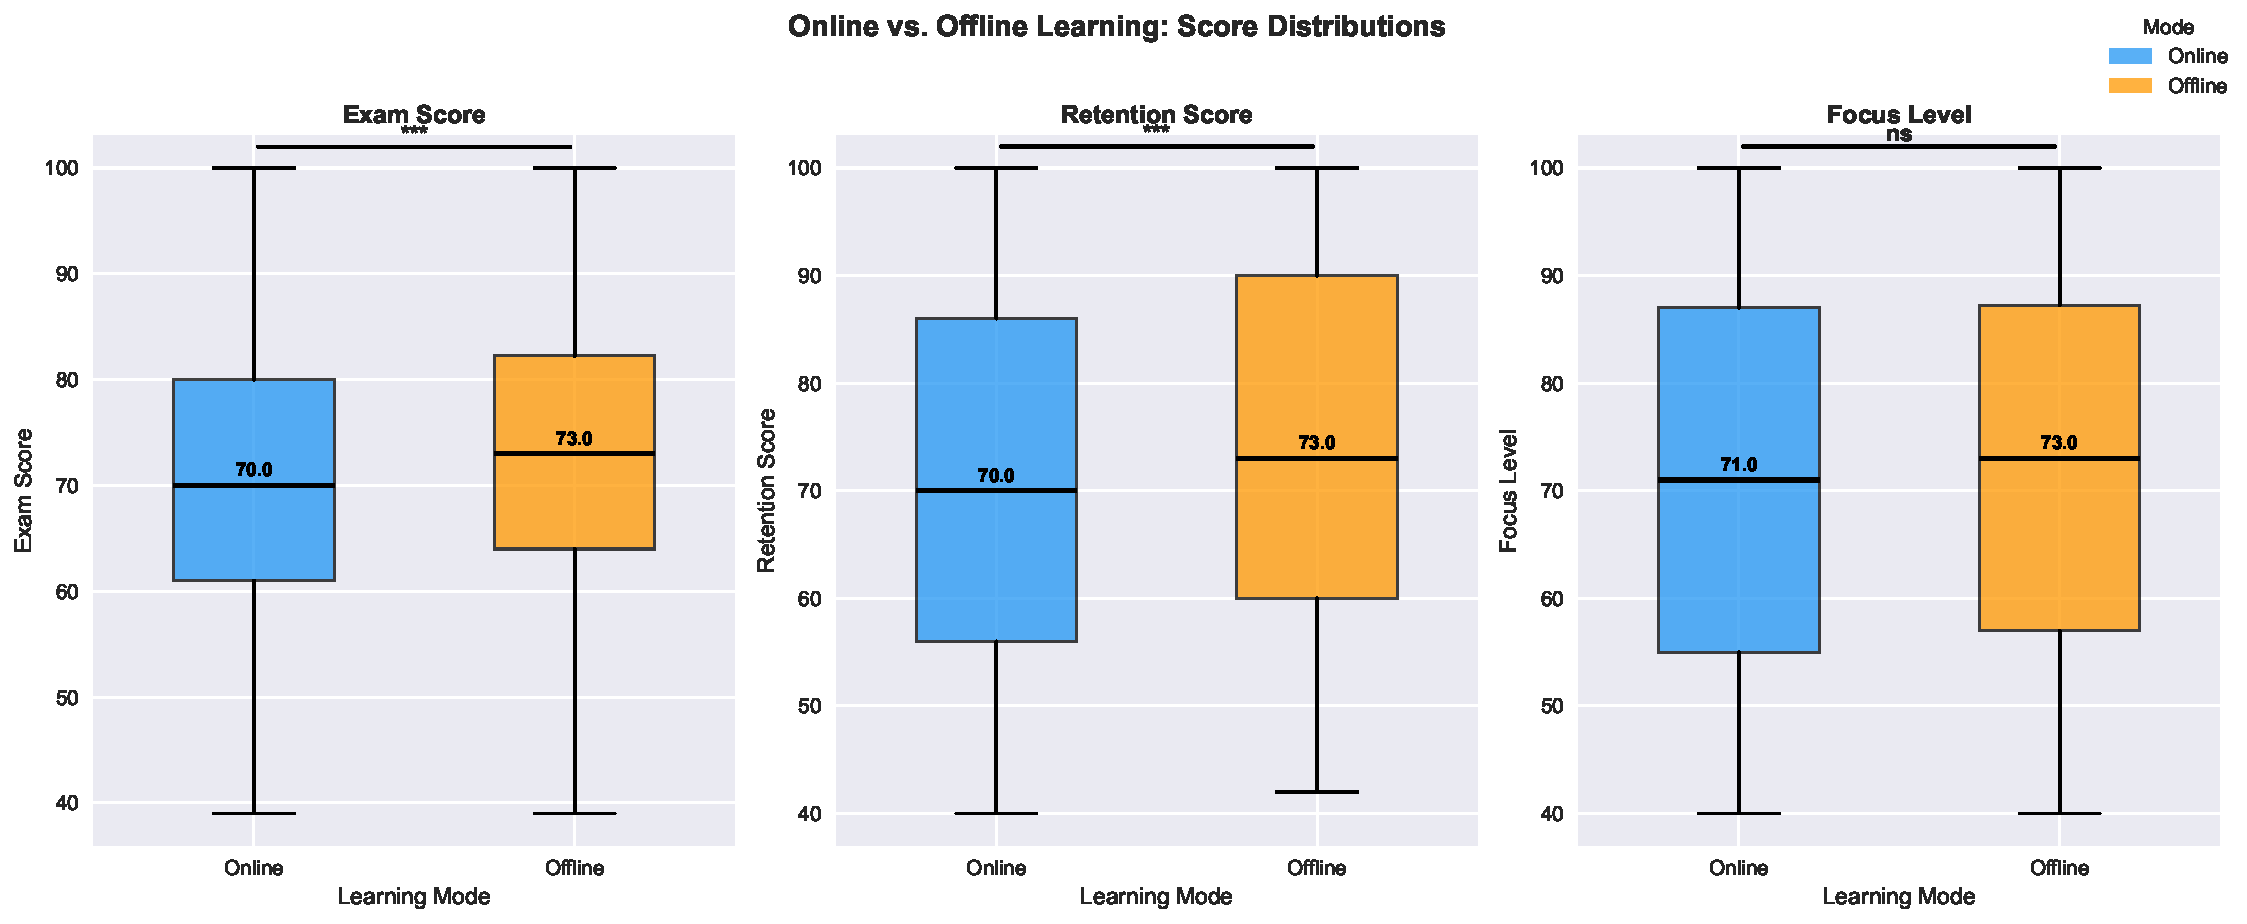
\includegraphics[width=0.95\textwidth]{fig1_score_distributions.pdf}
  \caption{Score distributions (Exam Score, Retention Score, and Focus Level)
           for online and offline learners. Violin plots show kernel density
           estimates; embedded box plots indicate median and interquartile range.}
  \label{fig:fig1}
\end{figure}

\subsection{Subject-Level Analysis}

Figure~\ref{fig:fig2} and Table~\ref{tab:subject} present mean Exam Scores
broken down by both subject and modality.
Offline students outperform their online counterparts in \textit{every} subject,
with gaps ranging from $1.49$ points in Math to $4.09$ points in History.
The consistency of this pattern across all five disciplines strengthens the
inference that the offline advantage is not subject-specific but rather reflects a
broader modality effect.

\begin{figure}[H]
  \centering
  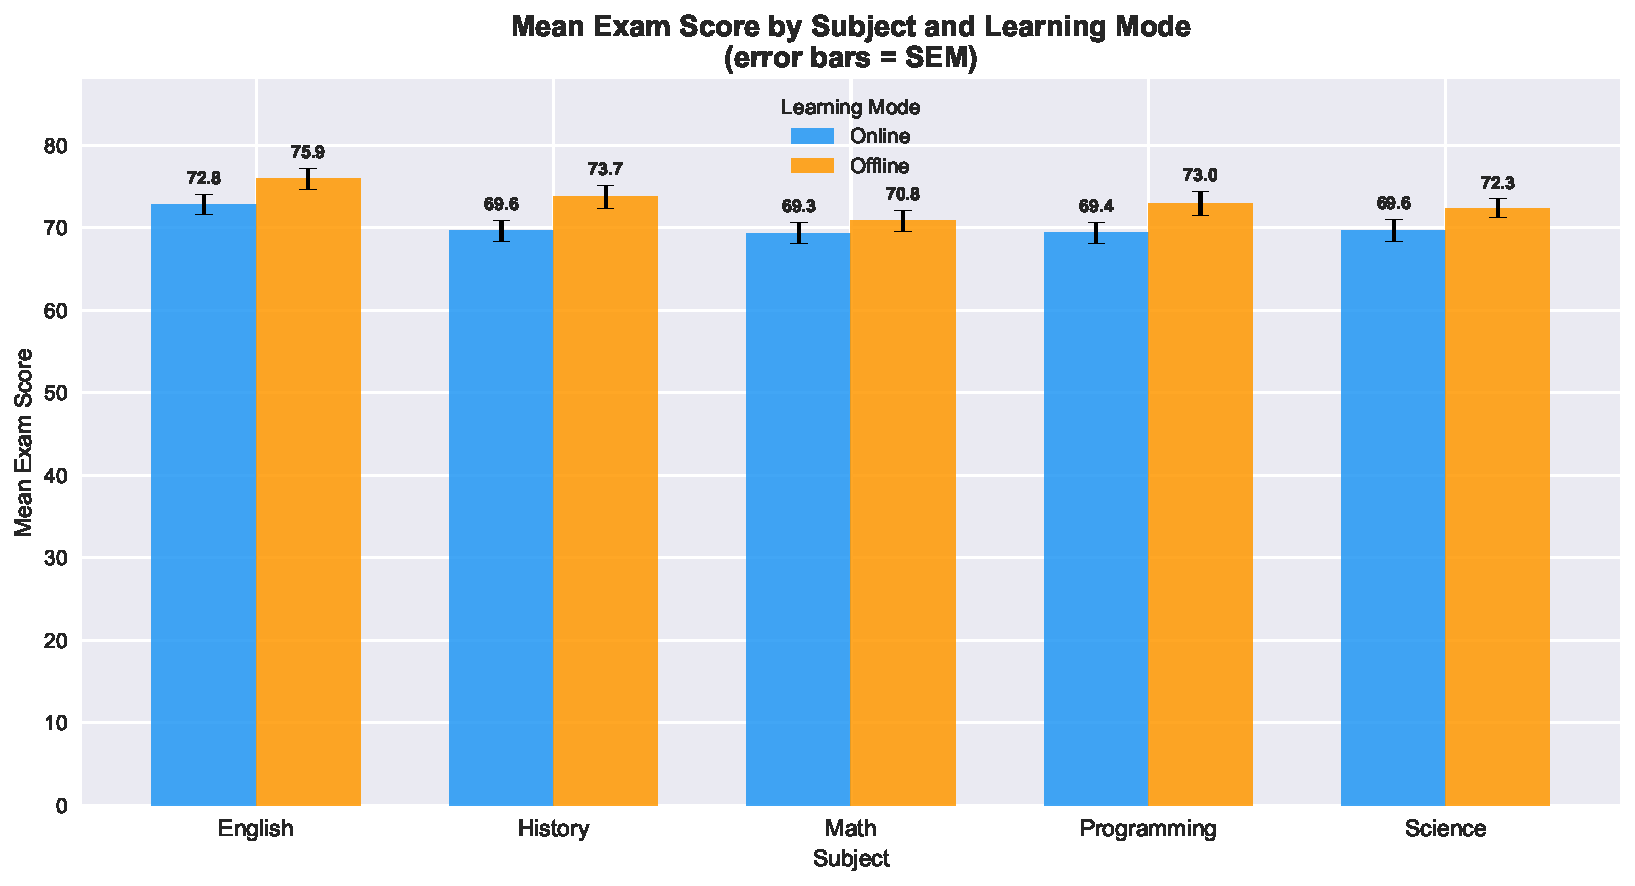
\includegraphics[width=0.95\textwidth]{fig2_exam_by_subject.pdf}
  \caption{Mean Exam Score by subject and learning modality.
           Error bars represent $\pm 1$ standard error of the mean.}
  \label{fig:fig2}
\end{figure}

\begin{table}[H]
  \centering
  \caption{Mean Exam Score by subject and learning modality, with
           offline--online gap.}
  \label{tab:subject}
  \begin{tabular}{lccr}
    \toprule
    \textbf{Subject} & \textbf{Online} & \textbf{Offline}
                     & \textbf{Gap (Offline $-$ Online)} \\
    \midrule
    English     & $72.77$ & $75.89$ & $+3.12$ \\
    History     & $69.63$ & $73.72$ & $+4.09$ \\
    Math        & $69.33$ & $70.83$ & $+1.49$ \\
    Programming & $69.36$ & $72.98$ & $+3.62$ \\
    Science     & $69.64$ & $72.33$ & $+2.69$ \\
    \bottomrule
  \end{tabular}
\end{table}

\subsection{Predictors of Exam Score}

Figures~\ref{fig:fig3} and~\ref{fig:fig4} show scatter plots of Exam Score against
Retention Score and Focus Level, respectively, with separate panels or colour-coded
markers for online and offline students.

\begin{figure}[H]
  \centering
  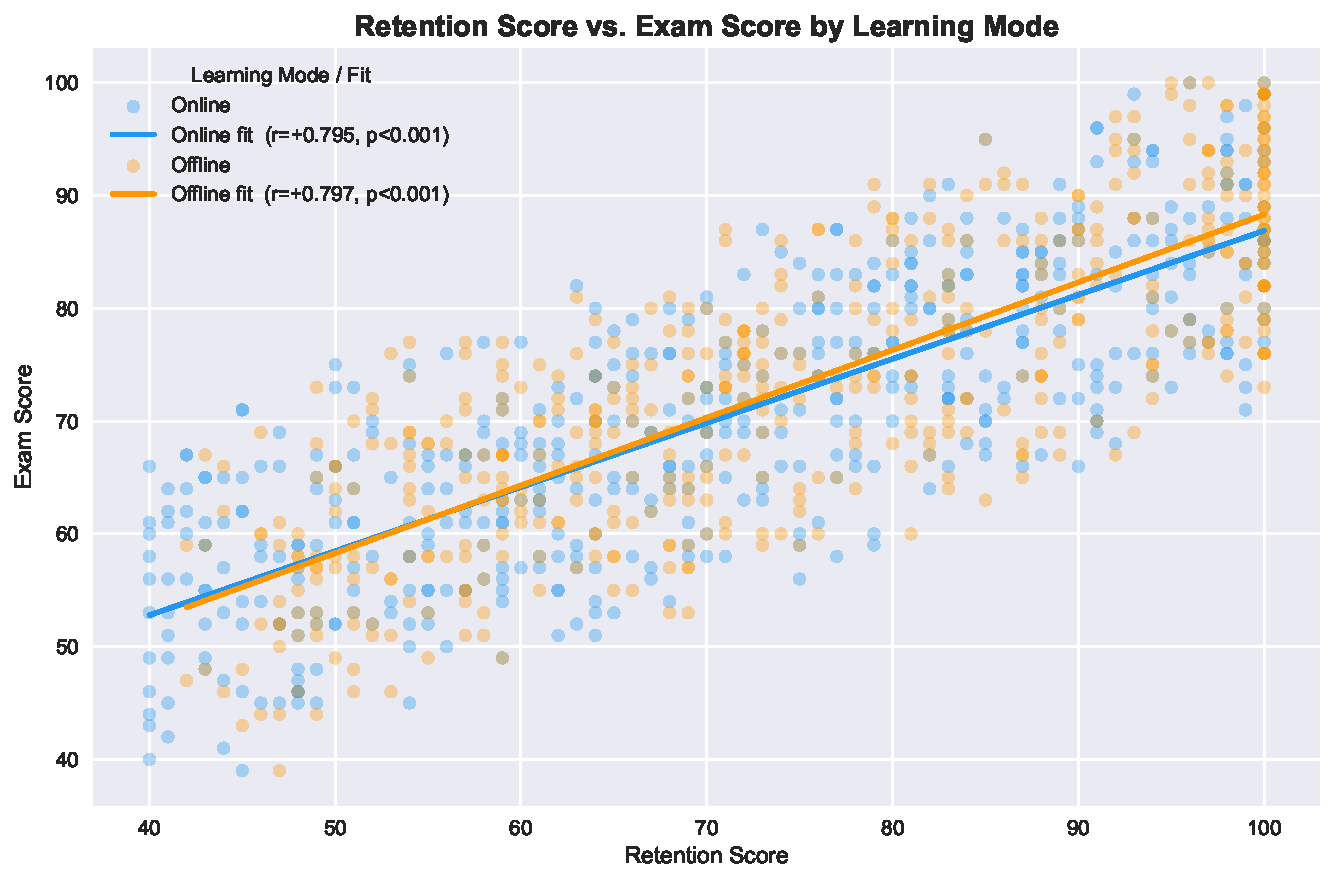
\includegraphics[width=0.95\textwidth]{fig3_retention_vs_exam.pdf}
  \caption{Scatter plot of Retention Score vs.\ Exam Score by modality.
           Regression lines are fitted separately for each group.
           The strong positive association is evident in both modalities.}
  \label{fig:fig3}
\end{figure}

\begin{figure}[H]
  \centering
  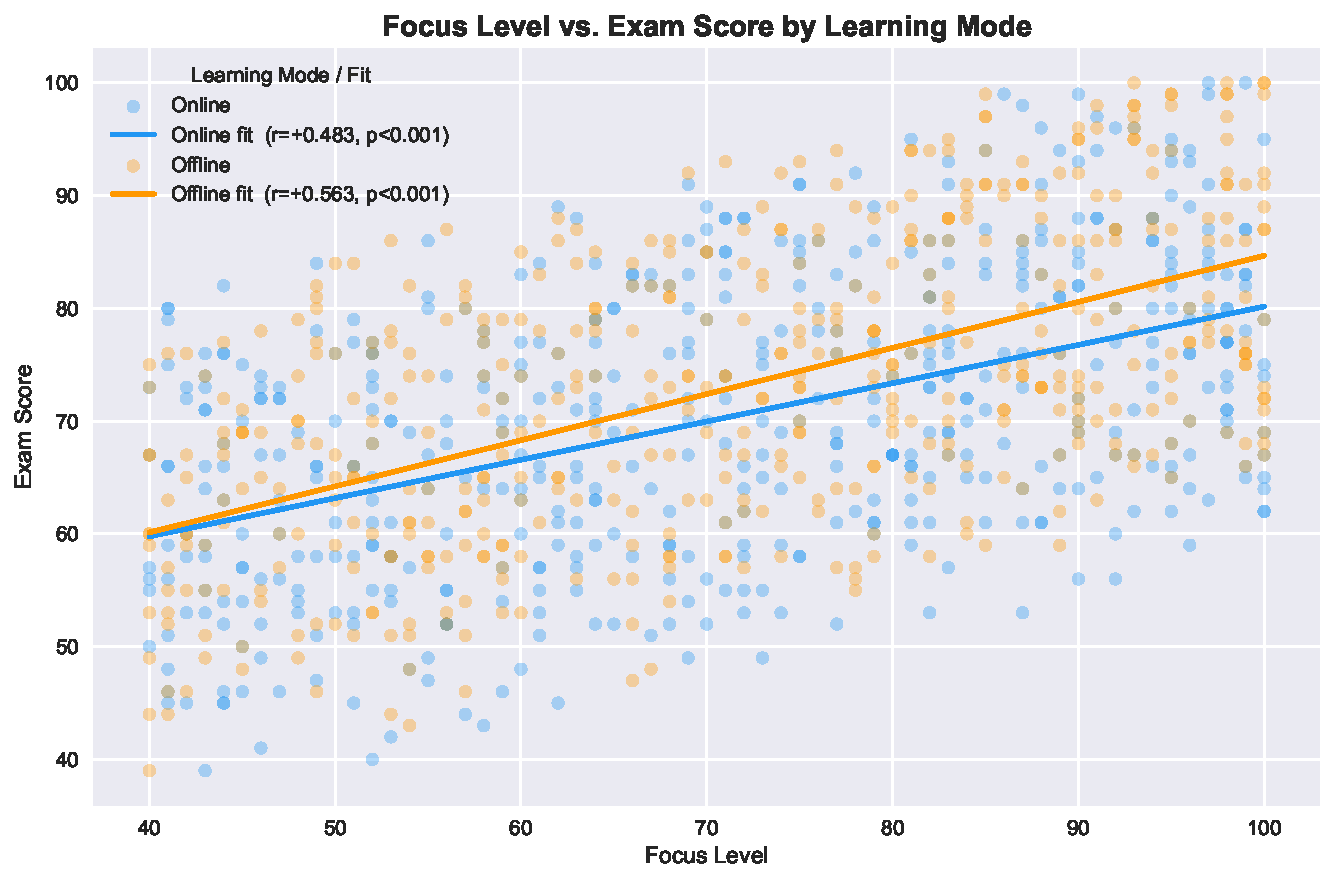
\includegraphics[width=0.95\textwidth]{fig4_focus_vs_exam.pdf}
  \caption{Scatter plot of Focus Level vs.\ Exam Score by modality.
           Regression lines are fitted separately for each group.
           The association is moderate and slightly stronger among offline students.}
  \label{fig:fig4}
\end{figure}

Table~\ref{tab:correlations} summarises Pearson correlations between Exam Score
and each predictor, stratified by modality.
Retention Score is the dominant predictor in both groups ($r \approx 0.80$,
$p < 0.001$), indicating that students who retain more course material
consistently achieve higher exam scores regardless of how they are taught.
Focus Level shows a moderate positive correlation that is somewhat stronger in the
offline group ($r = 0.5629$) than in the online group ($r = 0.4830$).
Study Hours displays a negligible and statistically non-significant association
with Exam Score in both modalities ($r = 0.0867$, $p = 0.053$ online;
$r = -0.0095$, $p = 0.833$ offline), suggesting that raw time investment alone
is a poor predictor of performance.

\begin{table}[H]
  \centering
  \caption{Pearson correlations with Exam Score, stratified by modality.
           All $p < 0.001$ unless stated otherwise.}
  \label{tab:correlations}
  \begin{tabular}{lcccc}
    \toprule
    & \multicolumn{2}{c}{\textbf{Online}} & \multicolumn{2}{c}{\textbf{Offline}} \\
    \cmidrule(lr){2-3} \cmidrule(lr){4-5}
    \textbf{Predictor} & $r$ & $p$ & $r$ & $p$ \\
    \midrule
    Retention\_Score & $0.7948$ & $< 0.001$ & $0.7970$ & $< 0.001$ \\
    Focus\_Level     & $0.4830$ & $< 0.001$ & $0.5629$ & $< 0.001$ \\
    Study\_Hours     & $0.0867$ & $0.053$   & $-0.0095$ & $0.833$ \\
    \bottomrule
  \end{tabular}
\end{table}

\subsection{Study Hours}

Figure~\ref{fig:fig5} displays the distribution of weekly Study Hours for online
and offline students.
Both groups show similar right-skewed distributions concentrated between roughly
2 and 7 hours per week, consistent with the non-significant $t$-test result
($t = -1.039$, $p = 0.299$) and the near-zero correlations with Exam Score.
This pattern suggests that the \textit{quantity} of study time is largely
decoupled from examination performance in this sample; qualitative aspects of
study---such as active retrieval and focused engagement---may matter more.

\begin{figure}[H]
  \centering
  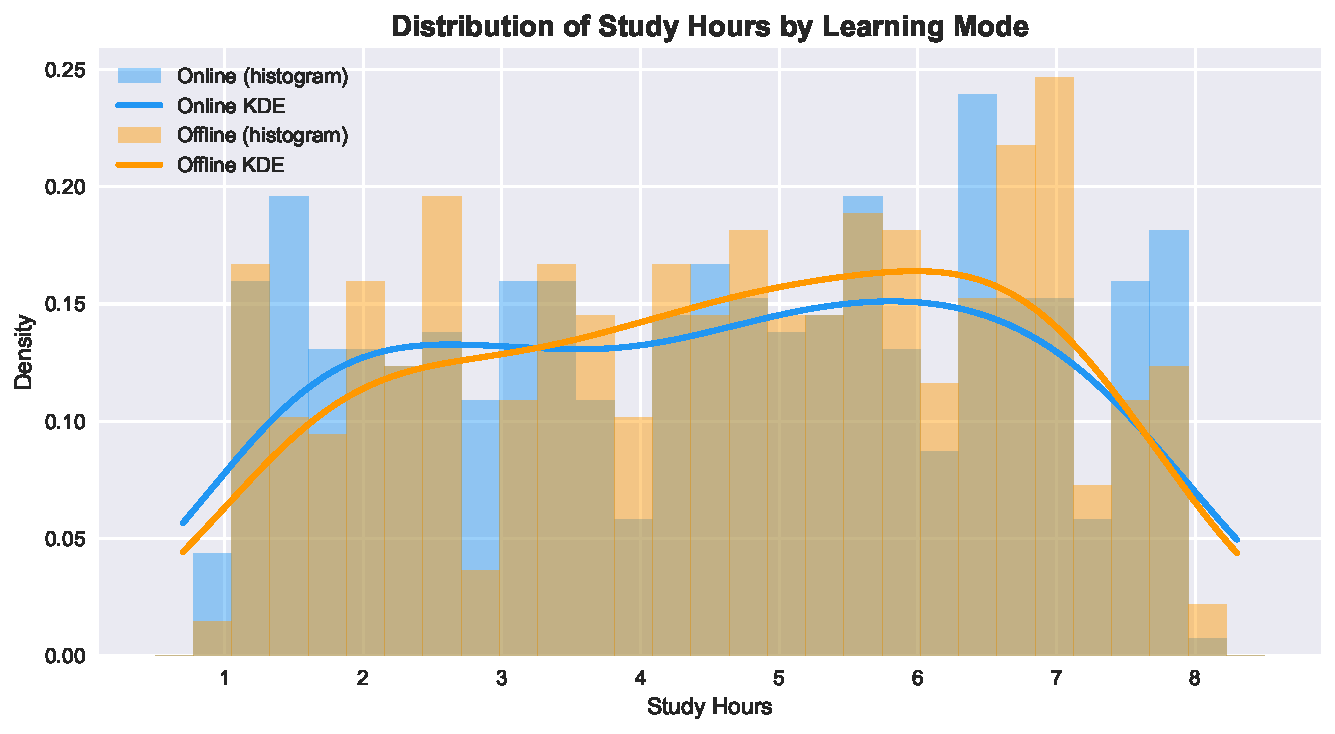
\includegraphics[width=0.85\textwidth]{fig5_study_hours_distribution.pdf}
  \caption{Distribution of weekly Study Hours by learning modality.
           Both groups exhibit similar distributions with comparable medians.}
  \label{fig:fig5}
\end{figure}

\subsection{Subject-Mode Heatmap}

Figure~\ref{fig:fig6} presents a heatmap of mean Exam Scores across the
subject-by-modality grid.
Warmer colours indicate higher mean scores.
The heatmap makes the subject-level offline advantage visually immediate:
every row (subject) shows a higher mean score in the offline column than in the
online column.
English in the offline modality yields the highest cell mean ($75.89$), while
Math online yields the lowest ($69.33$), a spread of approximately 6.6 points
across the full grid.

\begin{figure}[H]
  \centering
  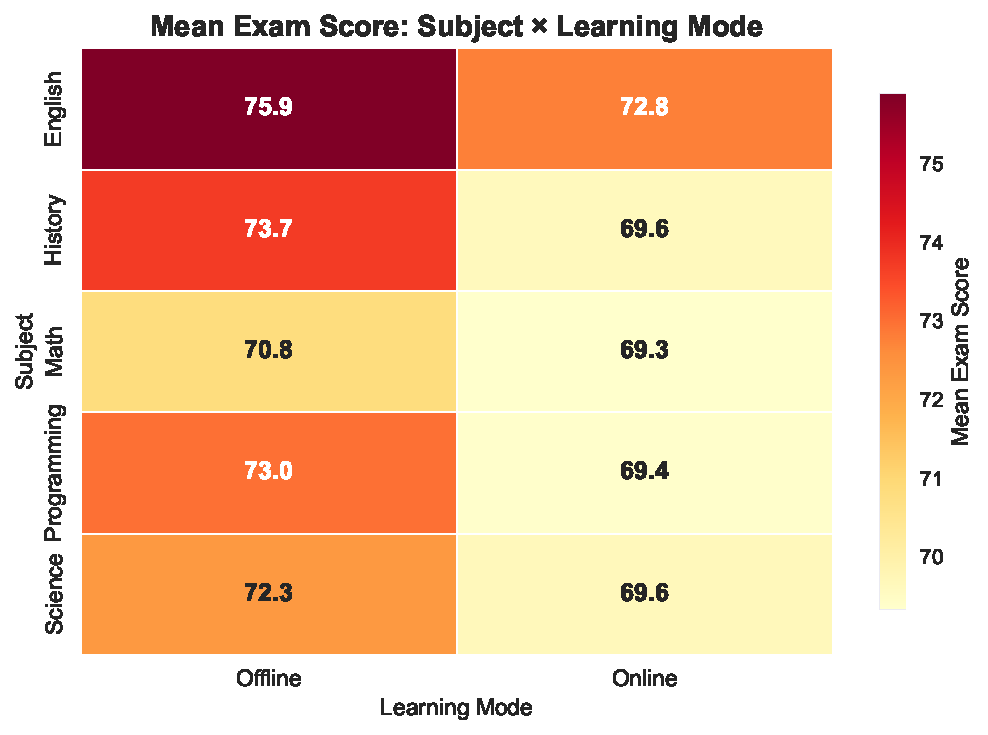
\includegraphics[width=0.75\textwidth]{fig6_subject_heatmap.pdf}
  \caption{Heatmap of mean Exam Score by subject and learning modality.
           Cell values are annotated; darker shading indicates higher performance.}
  \label{fig:fig6}
\end{figure}

\section{Discussion}

\textbf{Exam performance and retention.}
The statistically significant offline advantage in both Exam Score
($\Delta = 2.93$ points, $p = 0.0004$) and Retention Score
($\Delta = 4.06$ points, $p = 0.0003$) is the central finding of this study.
While the absolute magnitude of the difference is modest relative to the
within-group standard deviations ($\approx 13$ points for Exam Score),
the consistency across all five subjects---and the replication via the
non-parametric Mann-Whitney $U$ test---lends confidence that this is a
genuine modality effect rather than a sampling artefact.

The offline advantage in retention deserves particular attention because
Retention Score is the single strongest predictor of Exam Score in both groups
($r \approx 0.80$).
This suggests a plausible mechanism: offline instruction may facilitate deeper
encoding of information (through richer social interaction, real-time feedback,
and structured in-person schedules), which in turn produces higher retention
and, downstream, higher exam scores.

\textbf{Focus and study time.}
The absence of a significant group difference in Focus Level ($p = 0.347$) and
Study Hours ($p = 0.299$) indicates that online students are not simply
less attentive or less diligent.
Online and offline learners invest similar amounts of time and report similar
levels of focus.
The performance gap therefore cannot be attributed to motivational differences
in this sample.
Interventions targeting the \textit{quality} of learning---retrieval practice,
spaced repetition, or structured peer discussion---may be more effective for
closing the gap than interventions aimed at increasing raw study time.

\textbf{Subject-level heterogeneity.}
The offline advantage is present in every subject but varies in magnitude.
History shows the largest gap (4.09 points), potentially because historical
reasoning benefits more from classroom debate and contextualisation.
Math shows the smallest gap (1.49 points), possibly because mathematical problem
solving translates more readily to self-paced online practice.
These differences suggest that the optimal learning modality may be at least
partially domain-dependent, and that a blanket policy favouring one mode over
the other may be suboptimal.

\textbf{Predictor structure.}
The near-identical Retention Score correlations across modalities
($r_{\text{on}} = 0.7948$, $r_{\text{off}} = 0.7970$) indicate that the
process linking retention to exam performance is modality-invariant.
The slightly larger Focus--Exam correlation in the offline group
($r_{\text{off}} = 0.5629$ vs.\ $r_{\text{on}} = 0.4830$) may reflect the
more structured attentional demands of in-person classrooms.
The negligible role of Study Hours reinforces the well-established finding that
time on task is a necessary but not sufficient condition for academic achievement.

\textbf{Limitations.}
Several limitations should be acknowledged.
First, the dataset is a single cross-sectional snapshot; longitudinal data would
be needed to establish causal direction.
Second, it is unknown whether students self-selected into modalities, which could
introduce unmeasured confounds (e.g., prior achievement, motivation, internet
access).
Third, the Focus Level and Retention Score variables may carry measurement error
if they derive from self-report instruments.
Fourth, the analysis does not account for instructor effects, course design quality,
or platform differences within the online modality.
Future work should address these limitations through randomised or quasi-experimental
designs.

\section{Conclusion}

This study set out to answer three research questions; the findings provide clear
answers to each.

\textbf{RQ1} (Do online and offline students differ in Exam Score and Retention
Score?): \textit{Yes.}
Offline students score significantly higher on both outcomes
(Exam: $73.14$ vs.\ $70.21$, $p = 0.0004$;
Retention: $74.72$ vs.\ $70.66$, $p = 0.0003$).
The advantage is consistent across all five subjects, with subject-level gaps
ranging from 1.49 (Math) to 4.09 (History) points.

\textbf{RQ2} (Do Focus Level and Study Hours differ between modalities?):
\textit{No.}
Neither variable yields a statistically significant group difference
(Focus: $p = 0.347$; Study Hours: $p = 0.299$),
indicating that the learning-mode gap in outcomes is not driven by differences
in student effort or attention.

\textbf{RQ3} (Which variables best predict Exam Score within each modality?):
\textit{Retention Score is the dominant predictor in both groups} ($r \approx 0.80$),
followed by Focus Level ($r \approx 0.48$--$0.56$).
Study Hours is essentially unrelated to exam performance in both modalities.
The predictor structure is largely modality-invariant, suggesting that the
cognitive processes underpinning academic success operate similarly whether
students learn online or in person.

In sum, while online learning is a viable and accessible mode of instruction,
a meaningful performance gap---mediated largely by information retention---favours
offline learners in this dataset.
Practitioners designing or evaluating online programmes should prioritise
pedagogical strategies that strengthen retention, such as retrieval practice,
frequent low-stakes testing, and structured review sessions.

\end{document}
